\documentclass{article}
\usepackage{amsmath}
\usepackage{gensymb}
\usepackage{nicefrac}
\usepackage{multirow}
\usepackage{graphicx}
\usepackage[mathscr]{euscript}
\usepackage[margin=4cm]{geometry}



\title{\Huge{\sc{Swinging Atwood's \\ Machine}}}
\author{Michael Kister,  Alli Behr}
\date{}

\begin{document}
\maketitle

\section*{Introduction}

In our project, we investigated the behavior of the swinging Atwood's machine in the context of chaos theory.  We used the Hamiltonian from classical mechanics.  Once we found the differential equations, we explored the physics of the system with the use of a novel form of a bifurcation diagram as well as Poincar\'e maps.

\section*{Lagrangian Function}

Before beginning with our use of the Hamiltonian, we should first mention the Lagrangian functions, where the Lagrangian is defined as:

\begin{gather*}
\mathscr{L} = \mathscr{L}(q_{1}, \ldots, q_{n}, \dot{q_{1}}, \ldots, \dot{q_{n}}, t) = T - U \\
\end{gather*}

where:

\begin{gather*}
\frac{\partial \mathscr{L}}{\partial q_{i}} = \frac{d}{dt}\frac{\partial \mathscr{L}}{\partial \dot{q_{ix}}}
\end{gather*}

furthermore:

\begin{gather*}
p_{i} = \frac{\partial \mathscr{L}}{\partial \dot{q_{i}}}
\end{gather*}

\section*{Hamiltonian Function}

We now define the Hamiltonian to be:

\begin{gather*}
\mathscr{H} = \sum_{i = 1}^{n}p_{i}\dot{q_{i}} - \mathscr{L}
\end{gather*}

Noting that we want to keep:

\begin{gather*}
\mathscr{H} = \mathscr{H}(q_{1}, \ldots, q_{n}, p_{1}, \ldots, p_{n})
\end{gather*}

In our case, because we are dealing with a closed system and conservation of energy, we can say that:

\begin{gather*}
\mathscr{H} = T + U
\end{gather*}

where the Hamiltonian equations are:

\begin{gather*}
\dot{q}_{i} = \frac{\partial \mathscr{H}}{\partial p_{i}} \qquad\text{and}\qquad \dot{p_{i}} = - \frac{\partial \mathscr{H}}{\partial q_{i}}
\end{gather*}

\section*{Swinging Atwood's Machine}

For our system:

\begin{align*}
T &= \frac{1}{2}m_{1}v_{1}^{2}+\frac{1}{2}m_{1}v_{2}^{2} \\
&= \frac{1}{2}m_{1}\left( \dot{r_{1}}^{2} + (r_{1}\dot{\theta_{1}})^{2} \right) \,+\, \frac{1}{2}m_{2}\left( \dot{r_{2}}^{2} + (r_{2}\dot{\theta_{2}})^{2} \right) \\
U &= m_{1} \, g \, \left[ r_{1} \, (1-\cos{\theta_{1}}) + (R - r_{1}) \right] \,+\, m_{2} \, g \, \left[ r_{2} \, (1-\cos{\theta_{2}}) + (R - r_{2})\right]
\end{align*}

However, for our system, 

\begin{align*}
r_{2} = R - r_{1} \qquad&\text{and}\qquad \dot{r_{2}} = -\dot{r_{1}} \\
\dot{\theta_{2}} = 0 \qquad&\text{and}\qquad \theta_{2} = 0
\end{align*}

where $R$ is the combined length of the two string lengths.  Therefore, we say that

\begin{gather*}
\mathscr{H} = \frac{1}{2}m_{1}\left( \dot{r_{1}}^{2} + (r_{1}\dot{\theta_{1}})^{2} \right) \,+\, \frac{1}{2}m_{2}\dot{r}_{1}^{2} \,-\, m_{1}\,g\,r_{1}\,\cos{\theta_{1}} \,+\, m_{2}\,g\,r_{1} \\
\text{or} \\
\mathscr{H} = \frac{1}{2}m_{1}\left( \dot{r}^{2} + (r\,\dot{\theta})^{2} \right) \,+\, \frac{1}{2}m_{2}\,\dot{r}^{2} \,-\, m_{1}\,g\,r\,\cos{\theta} \,+\, m_{2}\,g\,r
\end{gather*}

Now we return to our requirement that $\mathscr{H}$ be in terms of $(q_{1}, \ldots, q_{n}, p_{1}, \ldots, p_{n})$.  To resolve this issue, we note that:

\begin{align*}
p_{r} = \frac{\partial \mathscr{L}}{\partial \dot{r}} &= \frac{\partial T}{\partial \dot{r}} \\
&= \frac{\partial}{\partial \dot{r}} \left( \frac{1}{2}m_{1}\left( \dot{r}^{2} + (r\,\dot{\theta})^{2} \right) \,+\, \frac{1}{2}m_{2}\,\dot{r}^{2} \right) \\
&= \dot{r}(m_{1} +m_{2}) \implies \\
\dot{r} &= \frac{p_{r}}{(m_{1}+m_{2})} \\
\\
&\text{and that:} \\
\\
p_{\theta} = \frac{\partial \mathscr{L}}{\partial \dot{\theta}} &= \frac{\partial T}{\partial \dot{\theta}} \\
&= \frac{\partial}{\partial \dot{\theta}}\left( \frac{1}{2}m_{1}\left( \dot{r}^{2} + (r\,\dot{\theta})^{2} \right) \,+\, \frac{1}{2}m_{2}\,\dot{r}^{2} \right) \\
&= m_{1} \, r^{2} \, \dot{\theta} \implies \\
\dot{\theta} &= \frac{p_{\theta}}{m_{1}\,r^{2}}
\end{align*}

We can thereby rewrite the Hamiltonian of the system as:

\begin{gather*}
\mathscr{H} = \frac{1}{2}m_{1}\left[ \left(\frac{p_{r}}{(m_{1}+m_{2})}\right)^{2} + \left(r\,\left(\frac{p_{\theta}}{m_{1}\,r^{2}}\right)\right)^{2} \right] \,+\, \frac{1}{2}m_{2}\,\left(\frac{p_{r}}{(m_{1}+m_{2})}\right)^{2} \,-\, m_{1}\,g\,r\,\cos{\theta} \,+\, m_{2}\,g\,r \\
\\
\text{which simplifies to:} \\
\\
\mathscr{H} = \frac{p_{r}^{2}}{2(m_{1}+m_{2})} \,+\, \frac{p_{\theta}^{2}}{2\,m_{1}\,r^{2}} \,+\, m_{2}\,g\,r \,-\, m_{1}\,g\,r\,\cos{\theta}
\end{gather*}

Using our Hamiltonian equations, we obtain:

\begin{align*}
\dot{\theta} = \frac{\partial \mathscr{H}}{\partial p_{\theta}} = \frac{p_{\theta}}{m_{1}\,r^{2}} \qquad&\qquad\qquad \dot{p_{\theta}} = -\frac{\partial \mathscr{H}}{\partial \theta} = -m_{1}\,g\,r\,\sin{\theta} \\
\dot{r} = \frac{\partial \mathscr{H}}{\partial p_{r}} = \frac{p_{r}}{(m_{1}+m_{2})} \qquad&\qquad\qquad \dot{p_{r}} = -\frac{\partial \mathscr{H}}{\partial r} = \frac{p_{\theta}^{2}}{m_{1}\,r^{3}} \,-\, m_{2}\,g \,+\, m_{1}\,g\,\cos{\theta} \\
\end{align*}

Which are the differential equations we solved when simulating the swinging Atwood's machine.

\section*{Trajectories}

Once we had the differential equations that characterized our system, we were able to solve them in ipython notebook.  Given an initial set of conditions, we were able to plot the trajectories of the smaller mass for a variety of mass ratios.  In Fig. \ref{comparison} we compare our results with those found on Wikipedia.

\begin{figure}
\centering
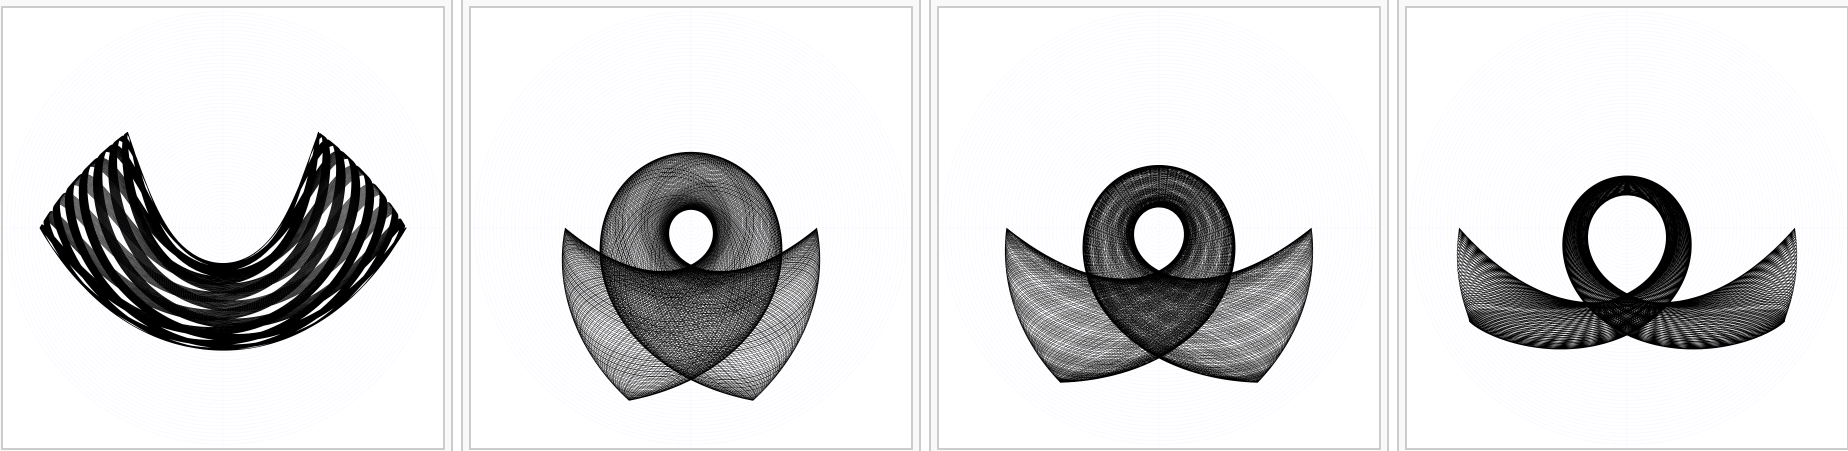
\includegraphics[width=\textwidth]{topper}
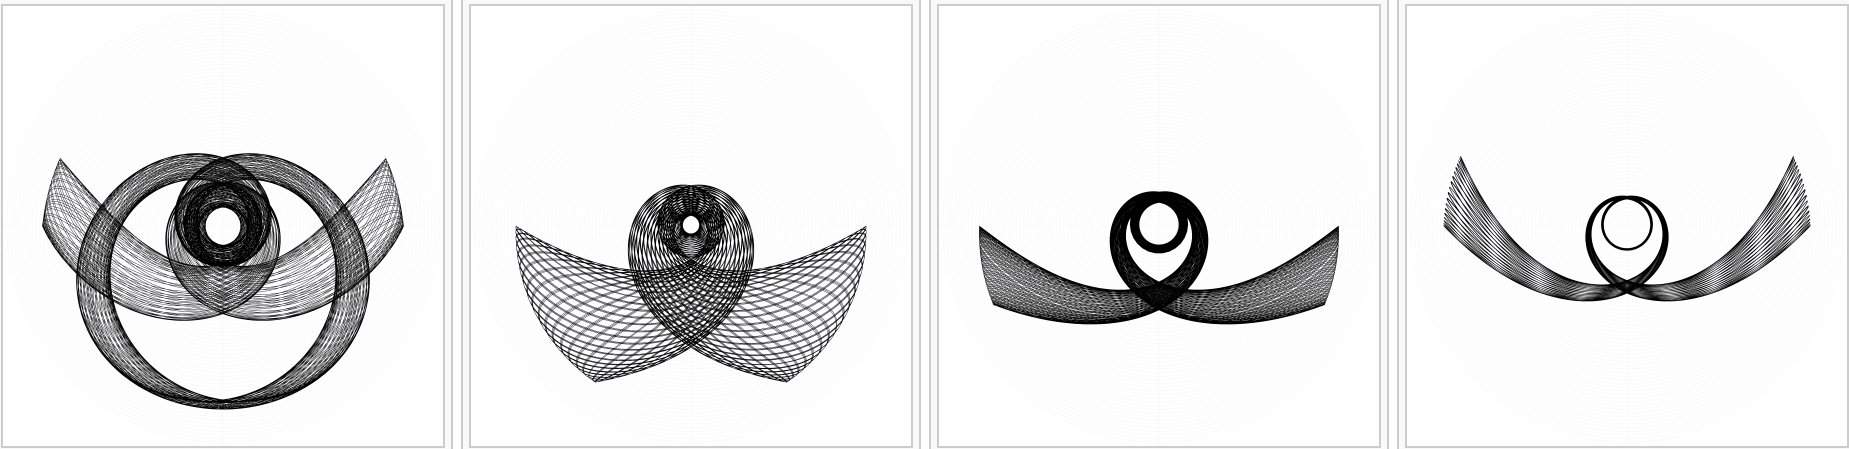
\includegraphics[width=\textwidth]{bottom}
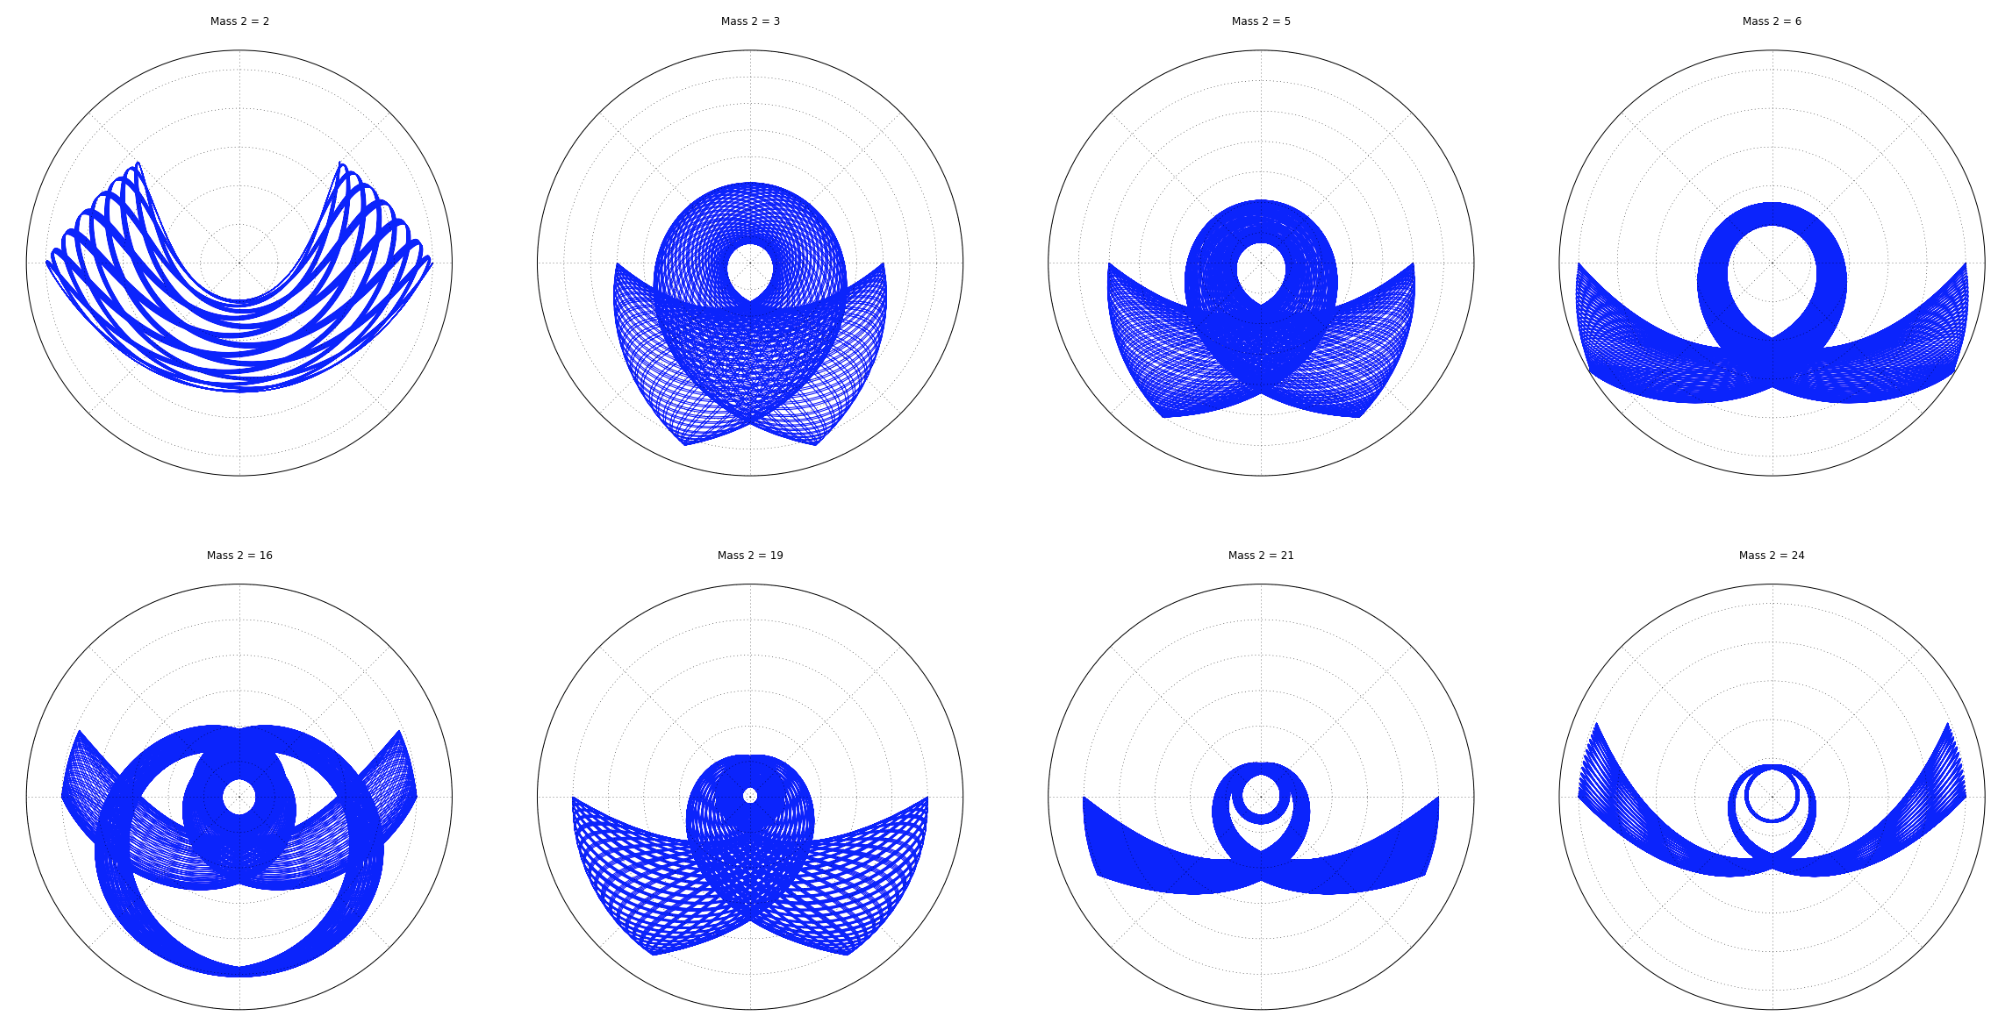
\includegraphics[width=\textwidth]{us}
\caption{We compare the plots proffered by Wikipedia (gray) with our plots (blue) for corresponding mass ratios.}
\label{comparison}
\end{figure}

From this comparison, we were able to convince ourselves that we were correctly solving the differential equations.

\section*{Bifurcation Diagram}

A bifurcation diagram shows the conditions achievable for a system for a varying value.  It is particularly useful for chaotic systems, where for many values of a variable, there are an infinite number of possible conditions.  For our system, we came up with a novel form of bifurcation diagram where we compared possible differences in adjacent orbits.

To achieve this analysis, we first identified points where the radius reached local maximum values.  We then noted that one ``period'' took place over the course of three of these maxima (one at the start, middle, and end).  So for adjacent periods we calculated the sum in the differences of corresponding $r_{i}(t)$ values, where $r_{i}(t)$ is the temporal dependence of radius for the $i$th period.  We calculated the sum of these differences for one hundred sets of adjacent periods for one thousand mass ratios, from which we obtained Fig. \ref{bifurcation}

\begin{figure}[h]
\centering
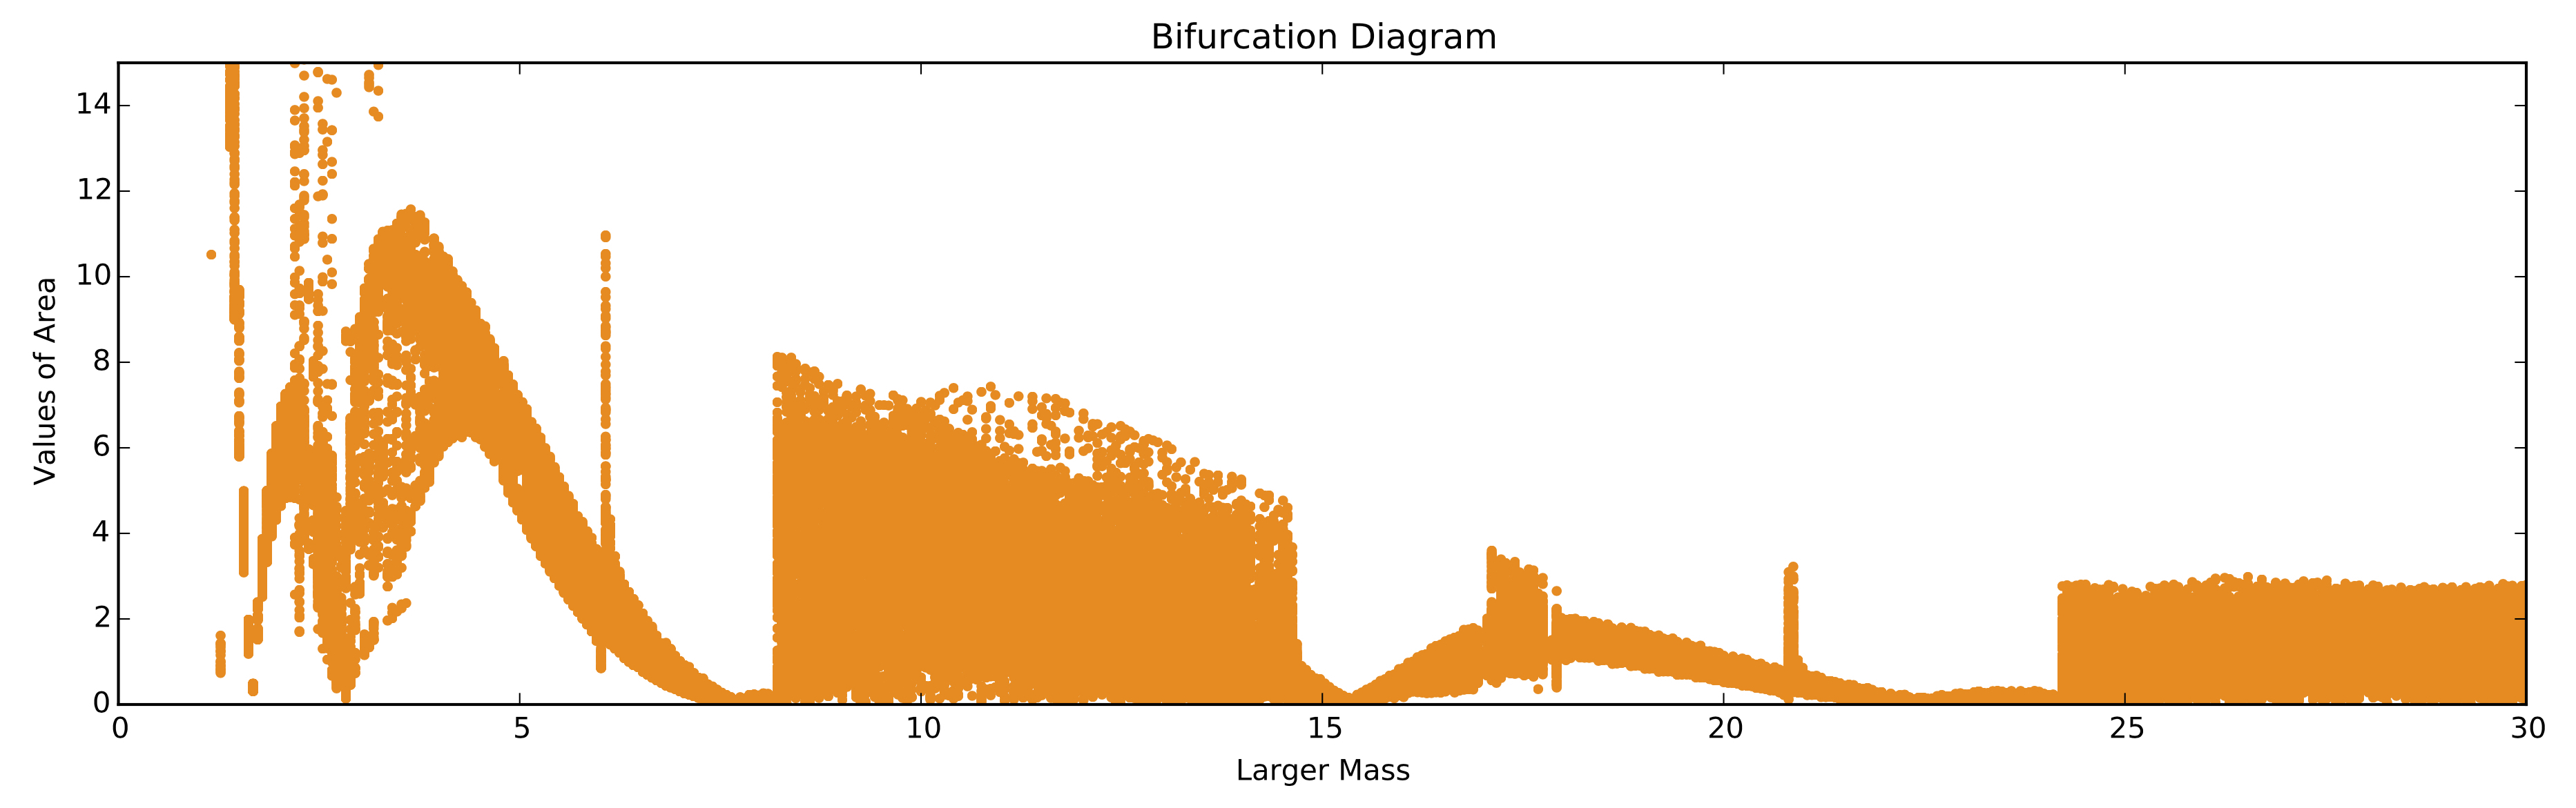
\includegraphics[width=\textwidth]{bifurcation}
\caption{Our approach to a bifurcation diagram.  Possible differences in orbits are plotted against a changing ratio of masses.}
\label{bifurcation}
\end{figure}

From Fig. \ref{bifurcation}, we can clearly see mass ratios where the possible differences in orbits are more varied than for other ratios.  The most notable examples of regions we could predict to be chaotic are between around 8 and 15, and past 24.  On the other hand, we can see areas of very similar orbits at locations such as 7.5 and 22.5.  In Fig. \ref{trajectories} we check the behavior of the system for mass ratios where the larger mass is 12 and 22.5 times larger than the smaller mass, and we can certainly see that the former is far more chaotic than the latter.

\begin{figure}
\centering
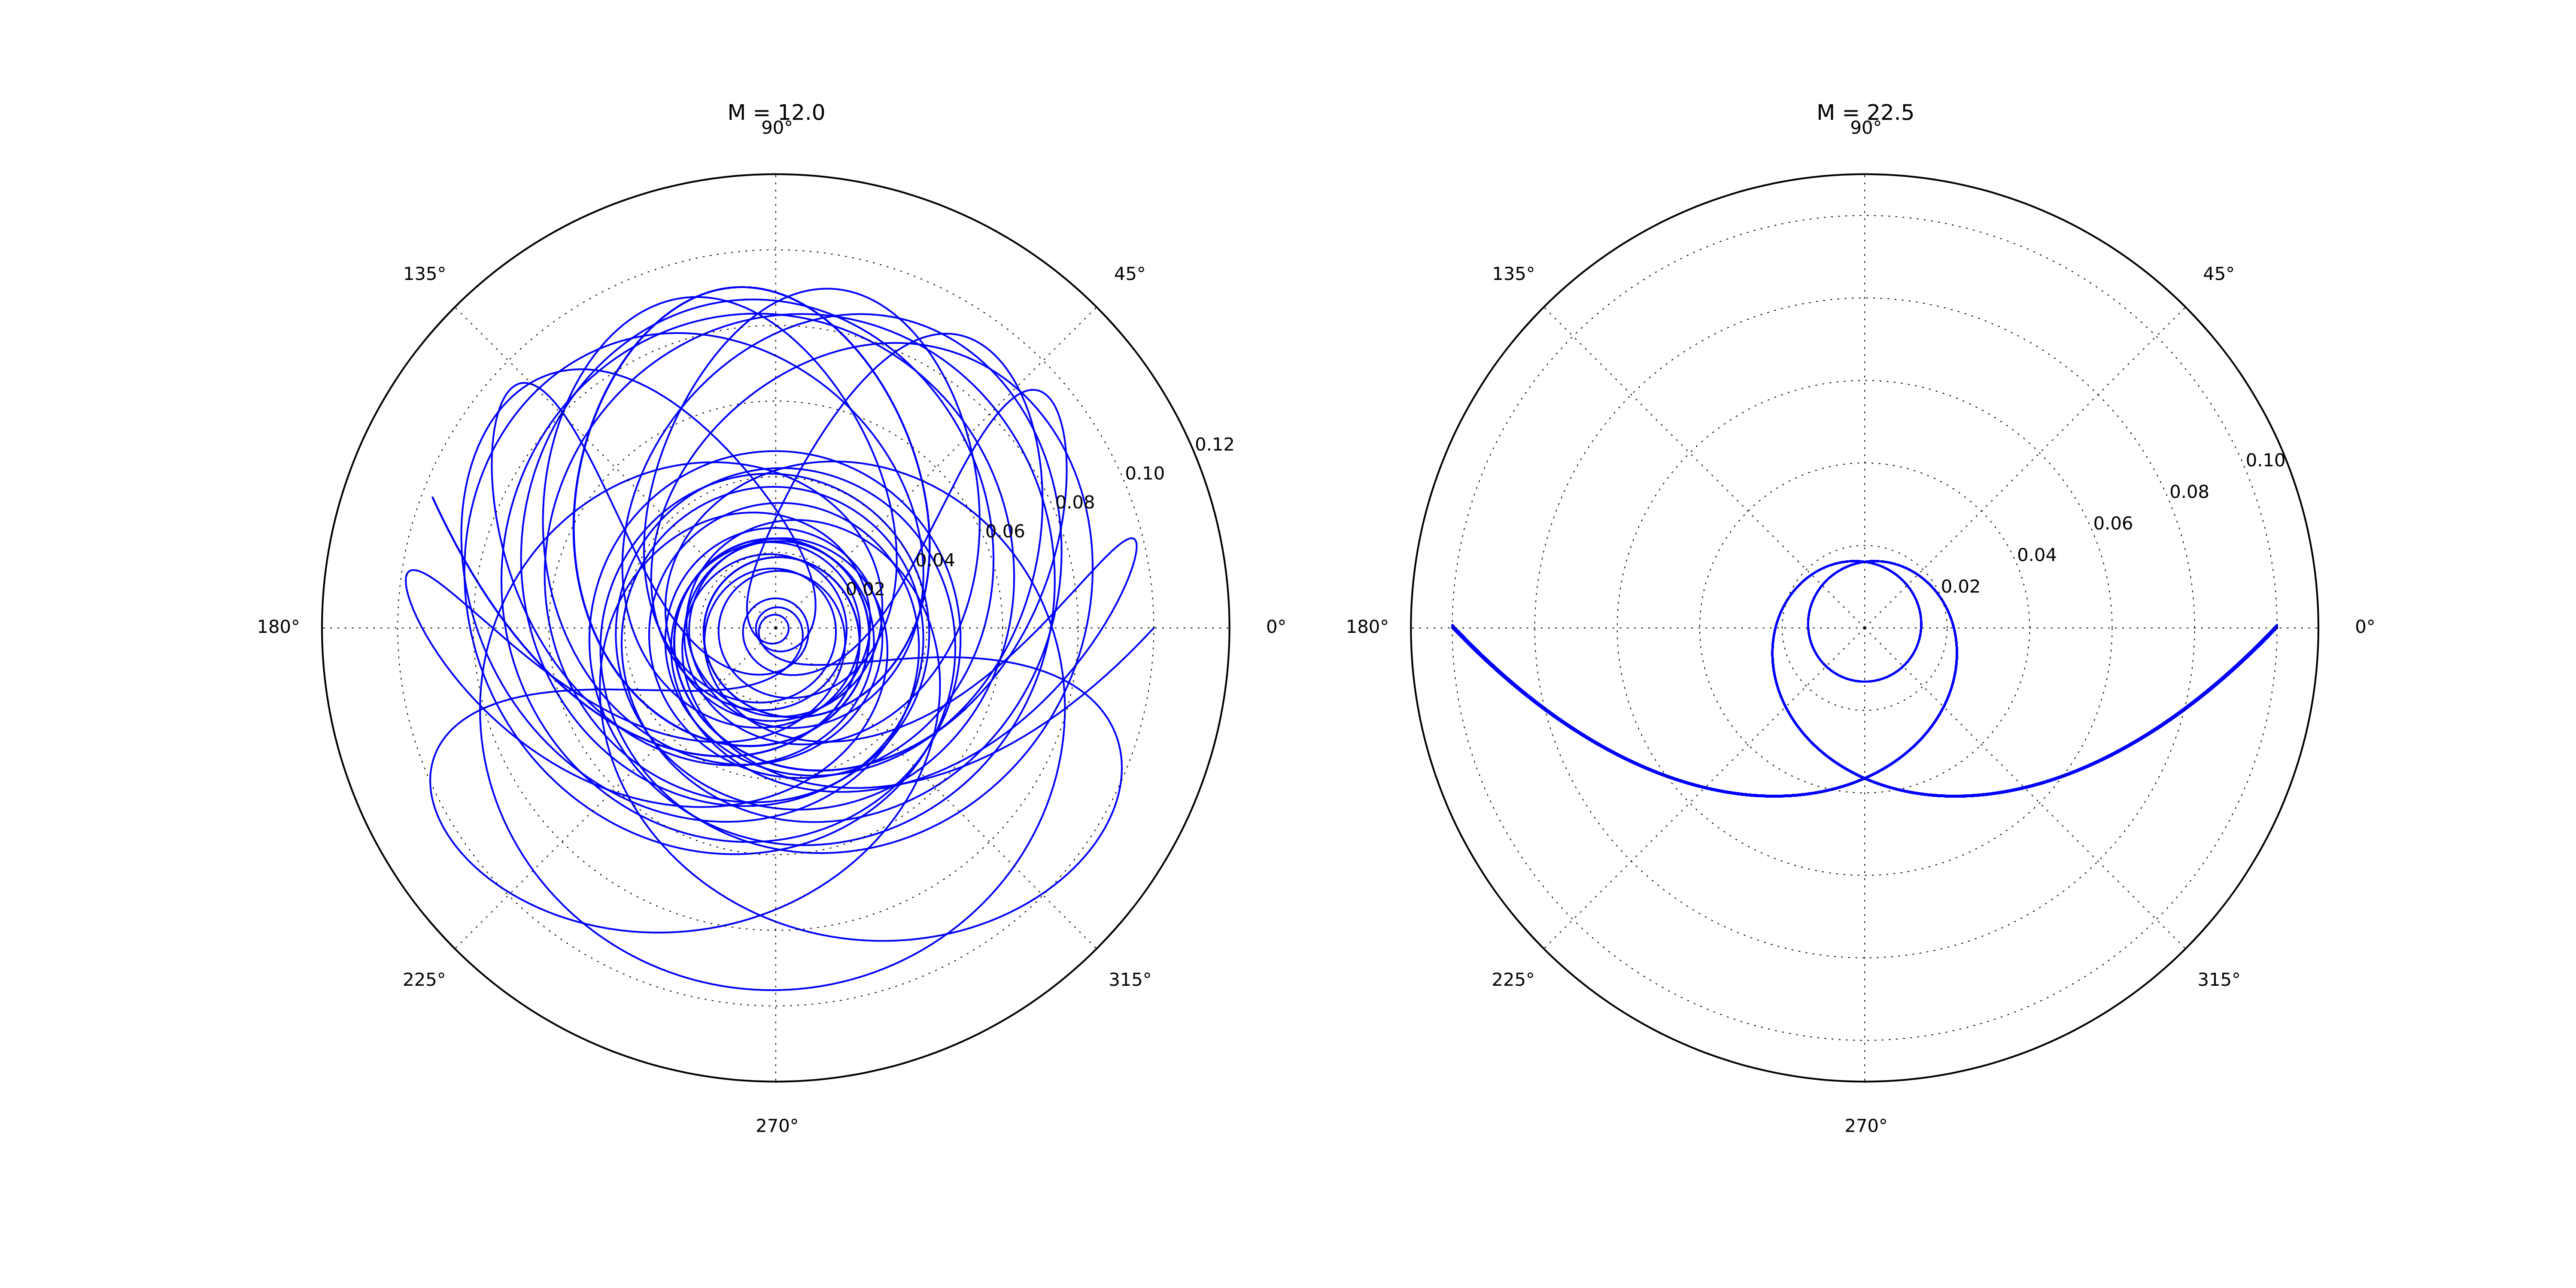
\includegraphics[width=\textwidth]{two_spots}
\caption{Two examples of trajectories.  The plot on the left is for a mass ratio of 12, and the plot on the right is for a mass ratio of 22.5.  These values were selected by using the bifurcation diagram to predict ratios that would be chaotic and non-chaotic.}
\label{trajectories}
\end{figure}

It should be noted that the system is not simply chaotic after $M/m > 24$, but continues to exit and re\"enter chaos for as long as we could see.

\section*{Phase Space}

Once we (numerically) solve our set of four differential equations for $r(t),\, \theta(t),\, p_{r}(t),\,\& \,\, p_{\theta}(t)$, we have what could be called a four-dimensional phase space.  However, since energy in our system is conserved (we are examining the case where the pulley is massless and frictionless), we can express any of the variables in terms of the other three.  Therefore, a plot containing information about three of these values is sufficient for describing the state of the system.

The idea of a Poincar\'e is ultimately to reduce the dimensionality of the phase space so it is possible to examine.  This is accomplished by examining two of the variables at points where the third variable is equal to a constant value.  For our data, we examined $p_r$ vs $r$, for locations where $\theta = 0$.  See Fig. \ref{nine_plots} for some examples of the Poincar\'e maps we achieved in our simulation.  

We note that these are different in appearance from some of the published maps, but ultimately we determined that since the sets of initial conditions were essentially infinite, and we were unable to find the precise conditions used in published works, that our differences rose from differing sets of initial conditions.

\section*{Lyapunov Exponents}

Lyapunov Exponents are the exponents used to classify how chaotic a system is.  These exponents specifically characterize the rate of separation of infinitesimally close trajectories in a dynamical system.  It was desired to find these exponents in order to confirm the behavior of our bifurcation diagram. The equation for the change in a trajectory over time is given by:

\begin{gather*}
|\delta Z(t)| \approx e^{{\lambda t}}|\delta Z_{0}|
\end{gather*}

where  $\lambda$ is the Lyapunov Exponent. This exponent gives an idea of the predictability of a system by giving the rate of separation of the trajectories. The maximum Lyapunov exponent for a system characterizes its overall behavior. If it is between 0 and 1, not including 0, it is considered chaotic and the greater it is, the more chaotic the system. The max Lyapunov exponent was found for our system using the equation:

\begin{gather*}
\lambda_{t} \approx \frac{1}{t}\ln{\frac{\delta Z_{t}}{\delta Z_{0}}}
\end{gather*}

to find the exponents for each time and finding the maximum of all these to find the max exponent for a specific mass.  This was done using the function  This exponent for each mass is plotted below using the function \texttt{lyapunovExponents}.  It is seen that the exponent is always positive, confirming the chaotic behavior of the machine. This plot has the same scale as our bifurcation diagram, so it can easily be compared. When done so, it is seen that as more chaos is shown on the bifurcation diagram, the exponent increases, suggesting that our bifurcation accurately portrays the system's chaos. 

\begin{figure}
\centering
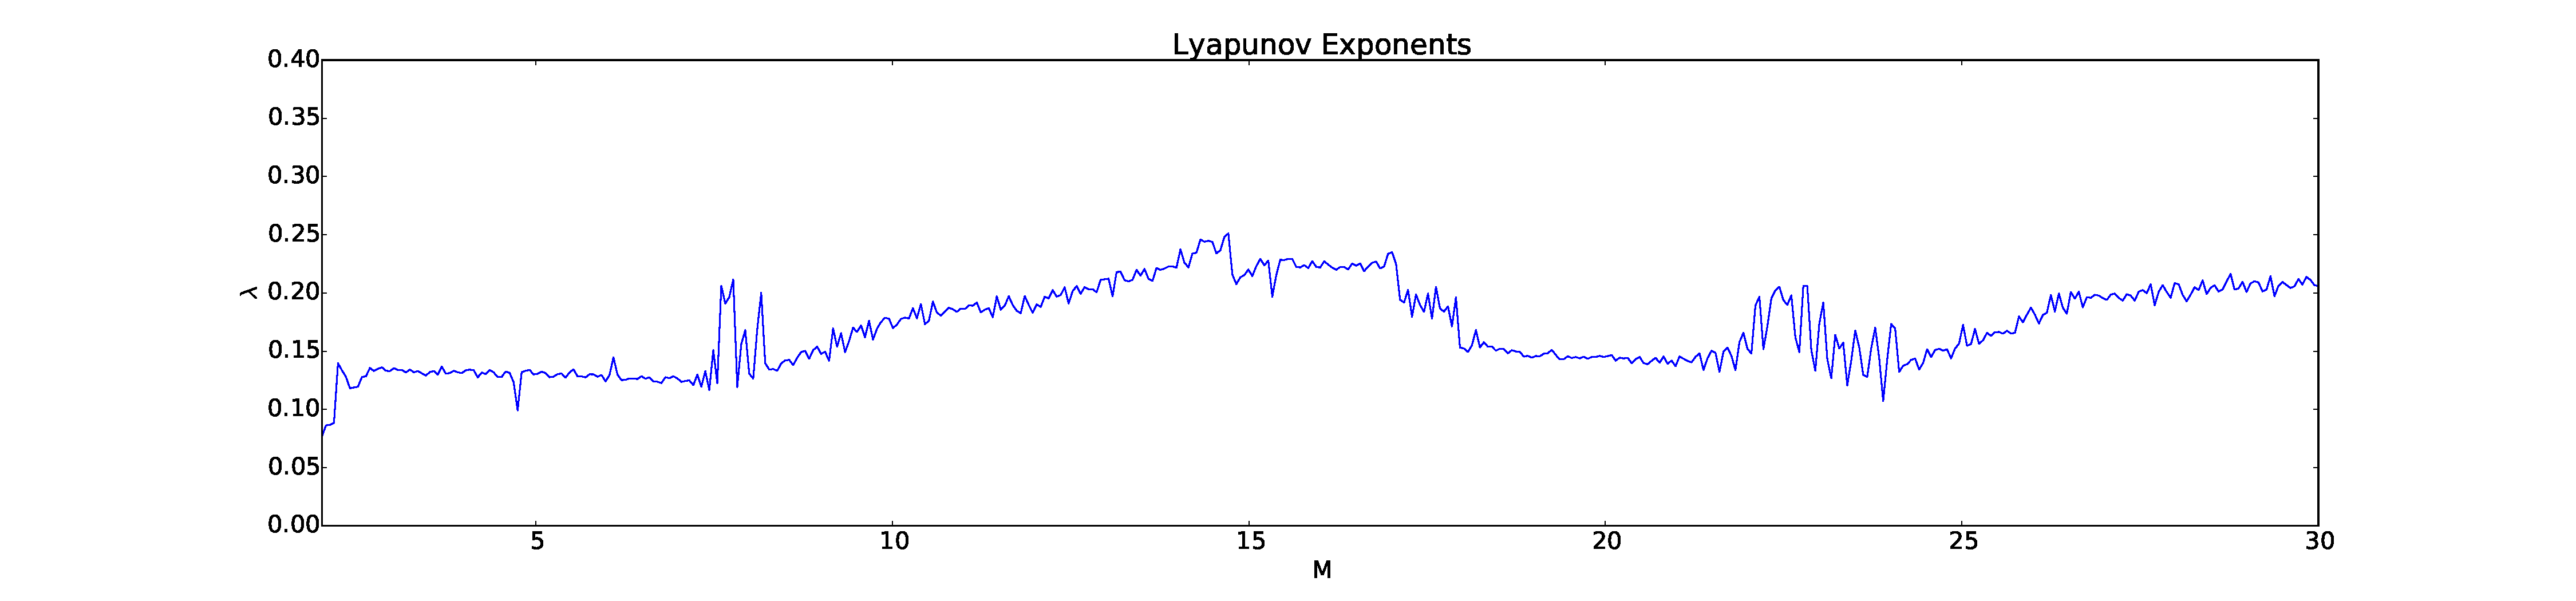
\includegraphics[width=\textwidth]{Lyapunov_2_30}
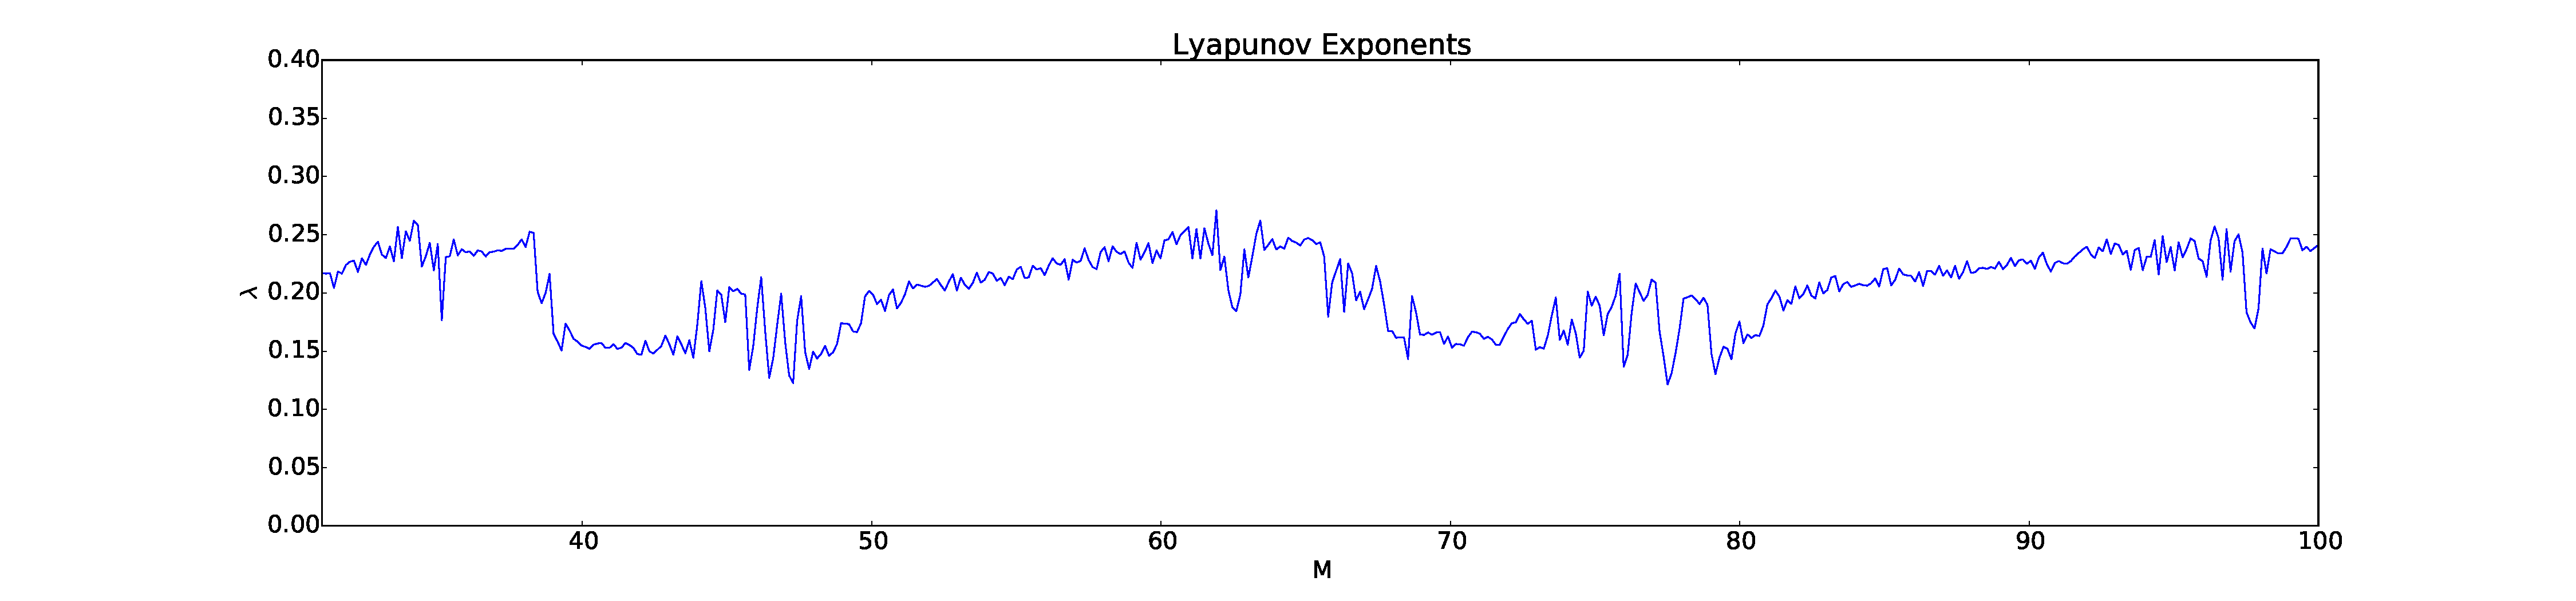
\includegraphics[width=\textwidth]{Lyapunov_31_100}
\caption{Here we show two excerpts of plotting the Lyapunov Exponent.  The upper plot shows the Lyapunov Exponent for $M \in \{1:30\}$, while the lower plot shows $M \in \{31:100\}$}
\label{lyapunovs}
\end{figure} 

\begin{figure}
\centering
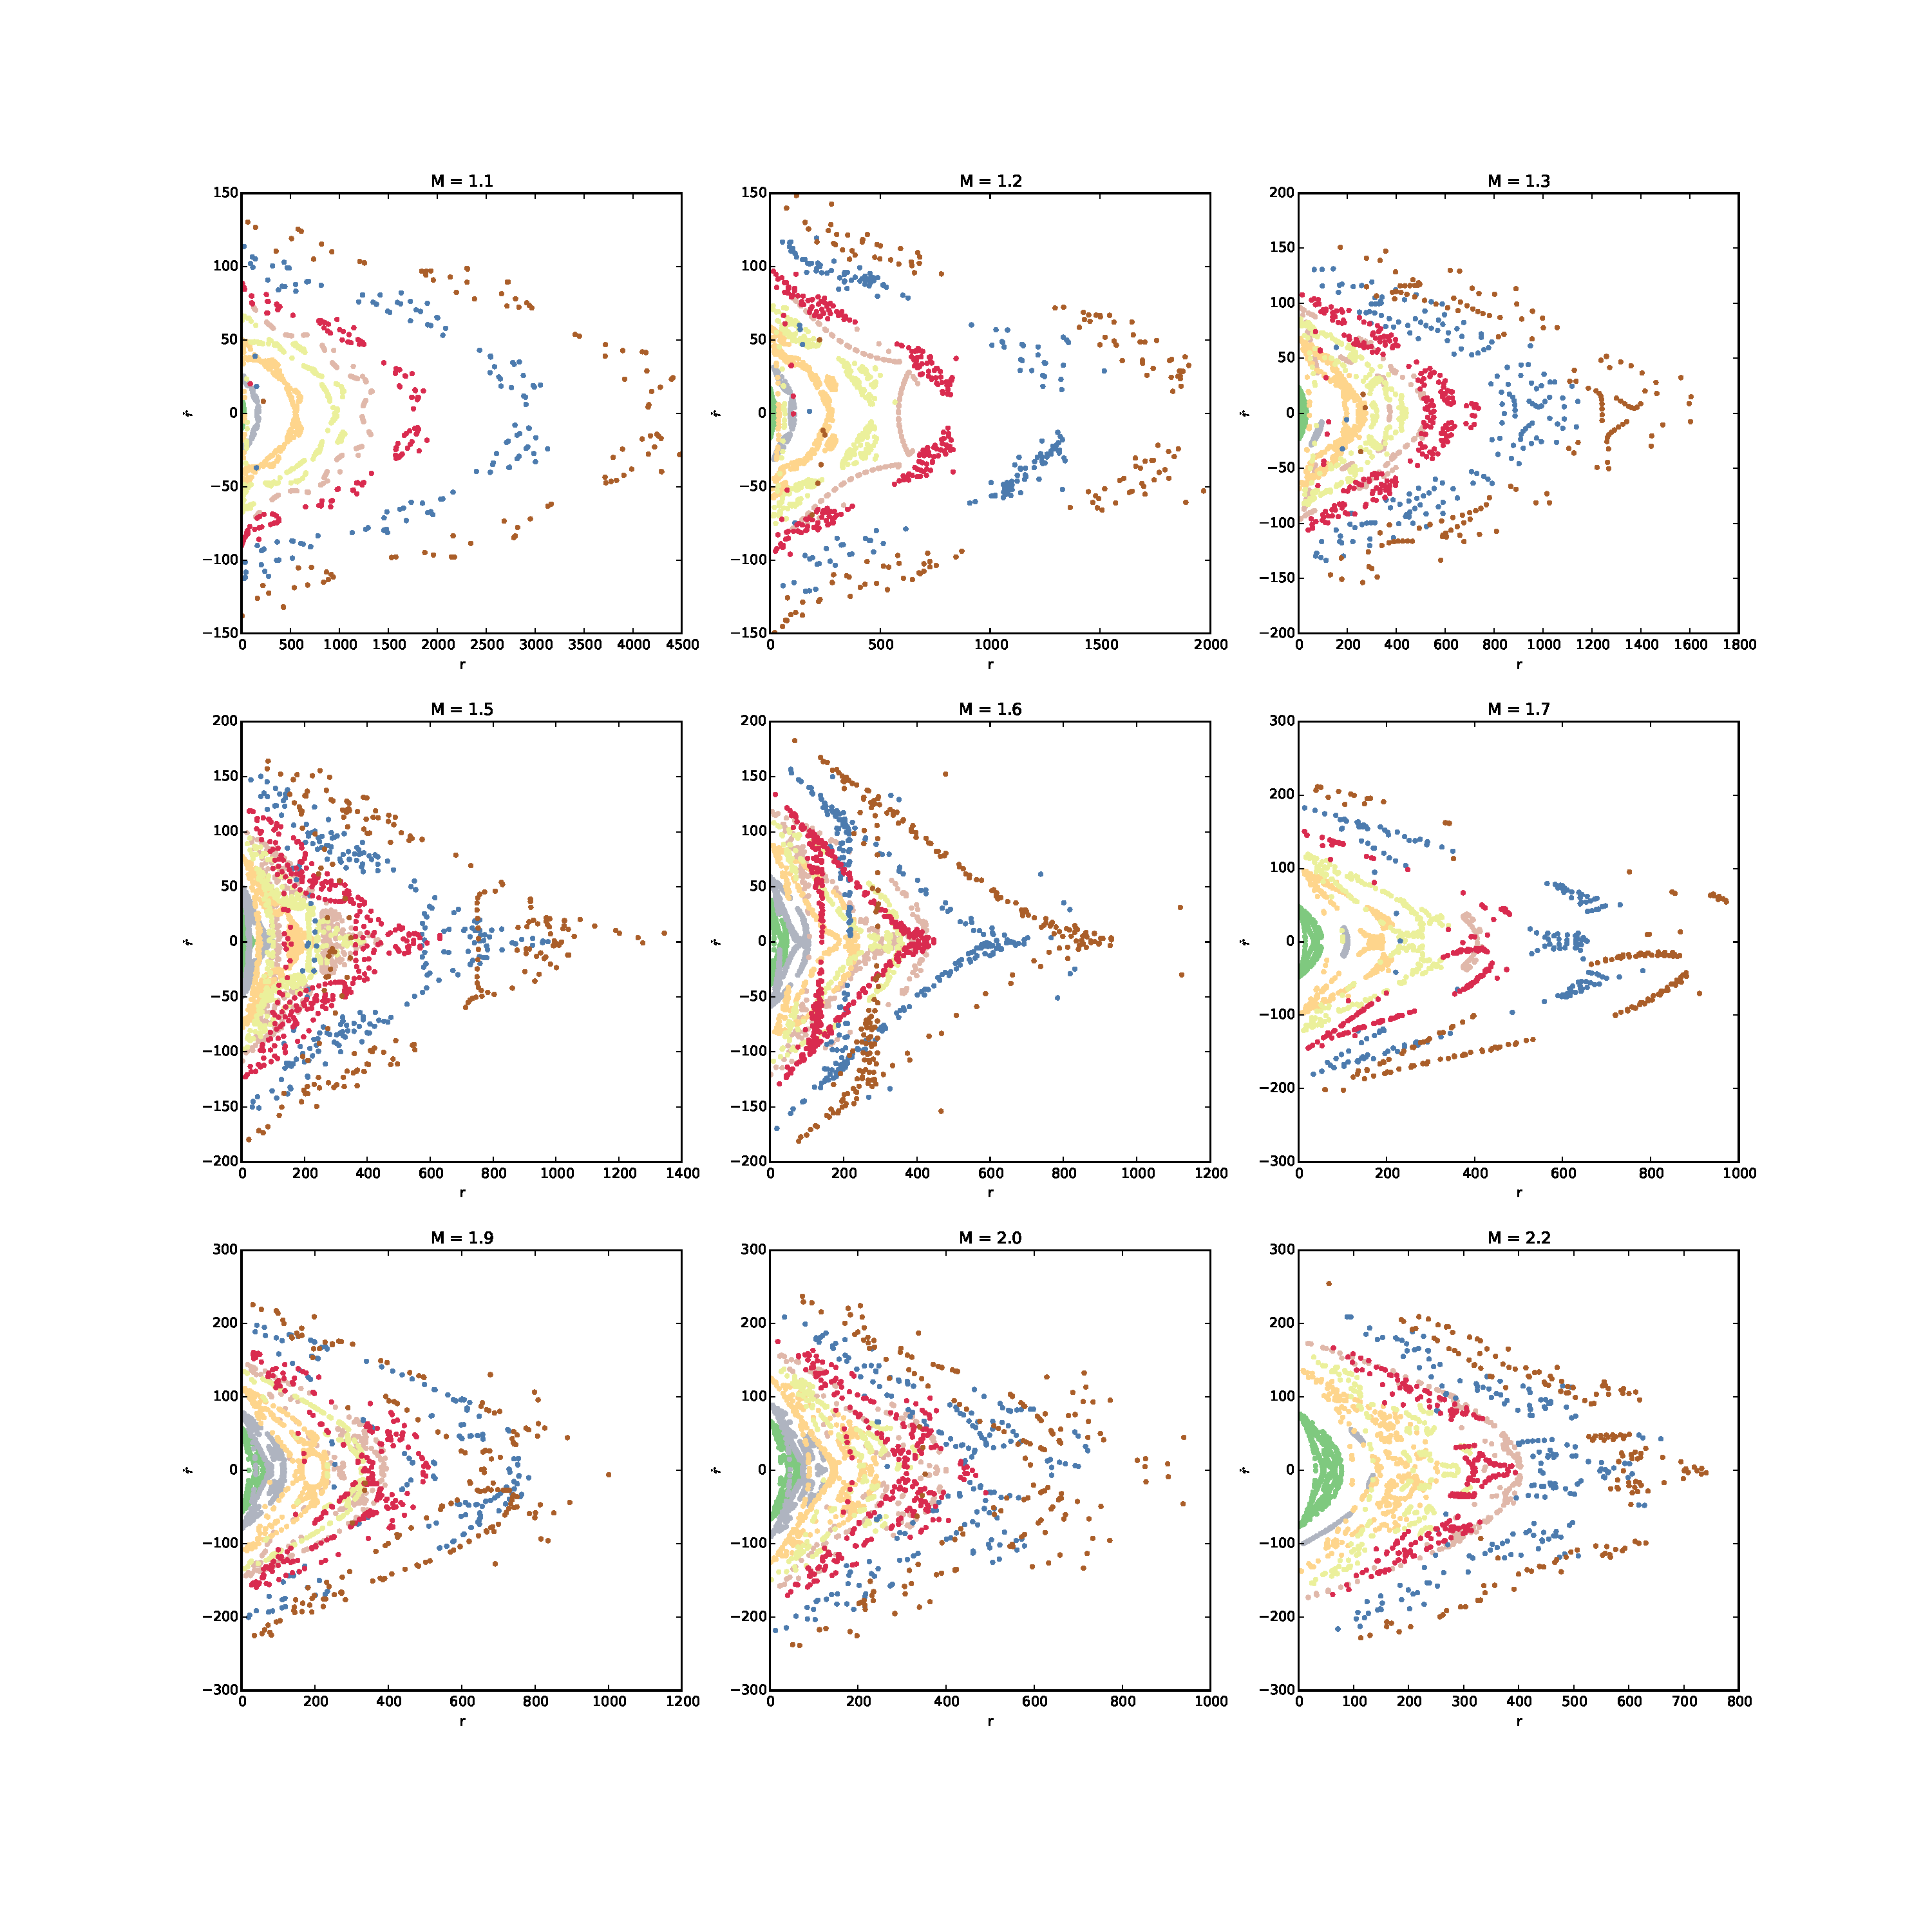
\includegraphics[width=\textwidth]{nine_plots}
\caption{Nine examples of Poincar\'e maps for different mass ratios, each with various initial conditions.}
\label{nine_plots}
\end{figure}

\section*{Conclusion}

Overall, we were satisfied with the information we could learn about the swinging Atwood's machine with the use of Python.  Whereas solving differential equations is useful way to find an analytic solution when possible, our numerical simulations provided more insight by exploring situations in which analytic solutions are not an option.  

One topic we remain curious about is an exploration of the system when it is not a closed system, for example when drag from the air, mass of the string, and friction of the string on the pulley are introduced.  This would afford us a more accurate portrayal of reality, but will require much more math.  We would also be interested in exploring how the concept of fractal dimensions plays a role in characterizing our phase plots.

\begin{thebibliography}{9}
\bibitem{first} 
Antonio Politi (2013) \texttt{http://www.scholarpedia.org/article Lyapunov\_exponent}
 
\bibitem{second} 
N. Tufillaro. Motions of a swinging Atwood's machine. \textit{Journal de Physique}, 1985, 46 (9),
	pp.1495-1500. 10.1051/jphys:019850046090149500. jpa-00210094
 
\bibitem{third} 
Swinging Atwood's machine. (2014, June 15). In Wikipedia, The Free Encyclopedia. Retrieved 05:43, 	December 2, 2015, from \texttt{https://en.wikipedia.org/w/index.php?title=Swinging\_Atwood}

\end{thebibliography}

\end{document}